\chapter{LAYER DECOMPOSITION}
Digital painting with different layers is an integral feature of digital image editing software. However, layers may never have existed for a scanned physical painting.Layers offer an intuitive way to edit the color and geometry of components and localize changes to the desired portion of the final image. Without layers, brush stroke segmentation becomes extremely challenging, since they can overlap and blend with each other.So,before extracting brush strokes, we decompose a Chinese painting into layers.\\
In our decomposition, each layer represents one coat of a painting with single color that is applied with varying opacity throughout the input painting. Wrong layer decomposition may cut one stroke into different layers. It is crucial to preserve the completeness and smoothness of the brush strokes in layer decomposition. To this end, we modify the layer decomposition algorithm in \cite{tan2016decomposing} by involving the coherent lines \cite{kang2007coherent} in our implementation. In the following we first address the layer decomposition algorithm \cite{tan2016decomposing} briefly and then discuss our modification. 


\section{Identify Paint Colors}

\begin{figure}[H]
	\centering
	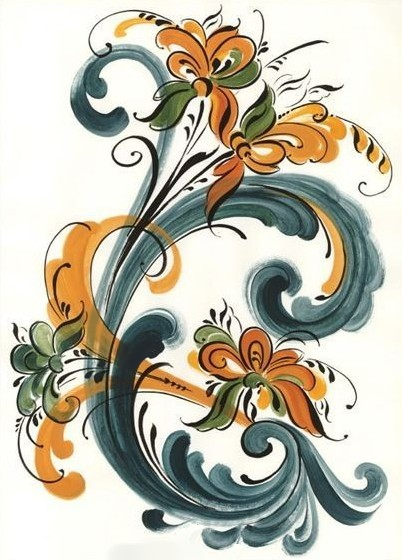
\includegraphics[height=0.2\textheight]{5.png}
	~~~~
	\includegraphics[height=0.2\textheight]{cube1.png}
	\caption{Geometry of input image pixels in RGB-space}
	\label{point cloud}
\end{figure}

In a brush painting, one region may have been painted multiply time with different paint colors. We assume that the color on each pixel is a linear combination of the paint colors, so all the pixel color in the input painting lies the convex hull of in the RGB space as showed in Figure \ref{point cloud} and Figure \ref{convex} , and every vertice is considered as a paint color. And base on such idea, we can represent each pixel color based on painted colors: 
\begin{equation*}
p=\Sigma \omega_i c_i
\end{equation*}
$p$ represents the color of the pixel, and $c_i$ represents the $i$-th paint color. 
To compute the paint color, we introduced the convex hull simplifying method of Tan's work \cite{tan2016decomposing}. In which a convex hull of the colors in RGB space should be computed, while every vertice is considered as a paint color. The colors would be tightly wrapped by the convex hull, but normally there would be many vertices more than what we need, since too many vertices would result in too many layers. In Tan's work \cite{tan2016decomposing} they provide a simplification method which would output manageable number of layers based on user need and the output layers with clearly differentiated colors,as showed in Figure \ref{convex}. And based on such method ,we generate a palette of paint colors of the input paintings. 

\begin{figure}[H]
	\centering
	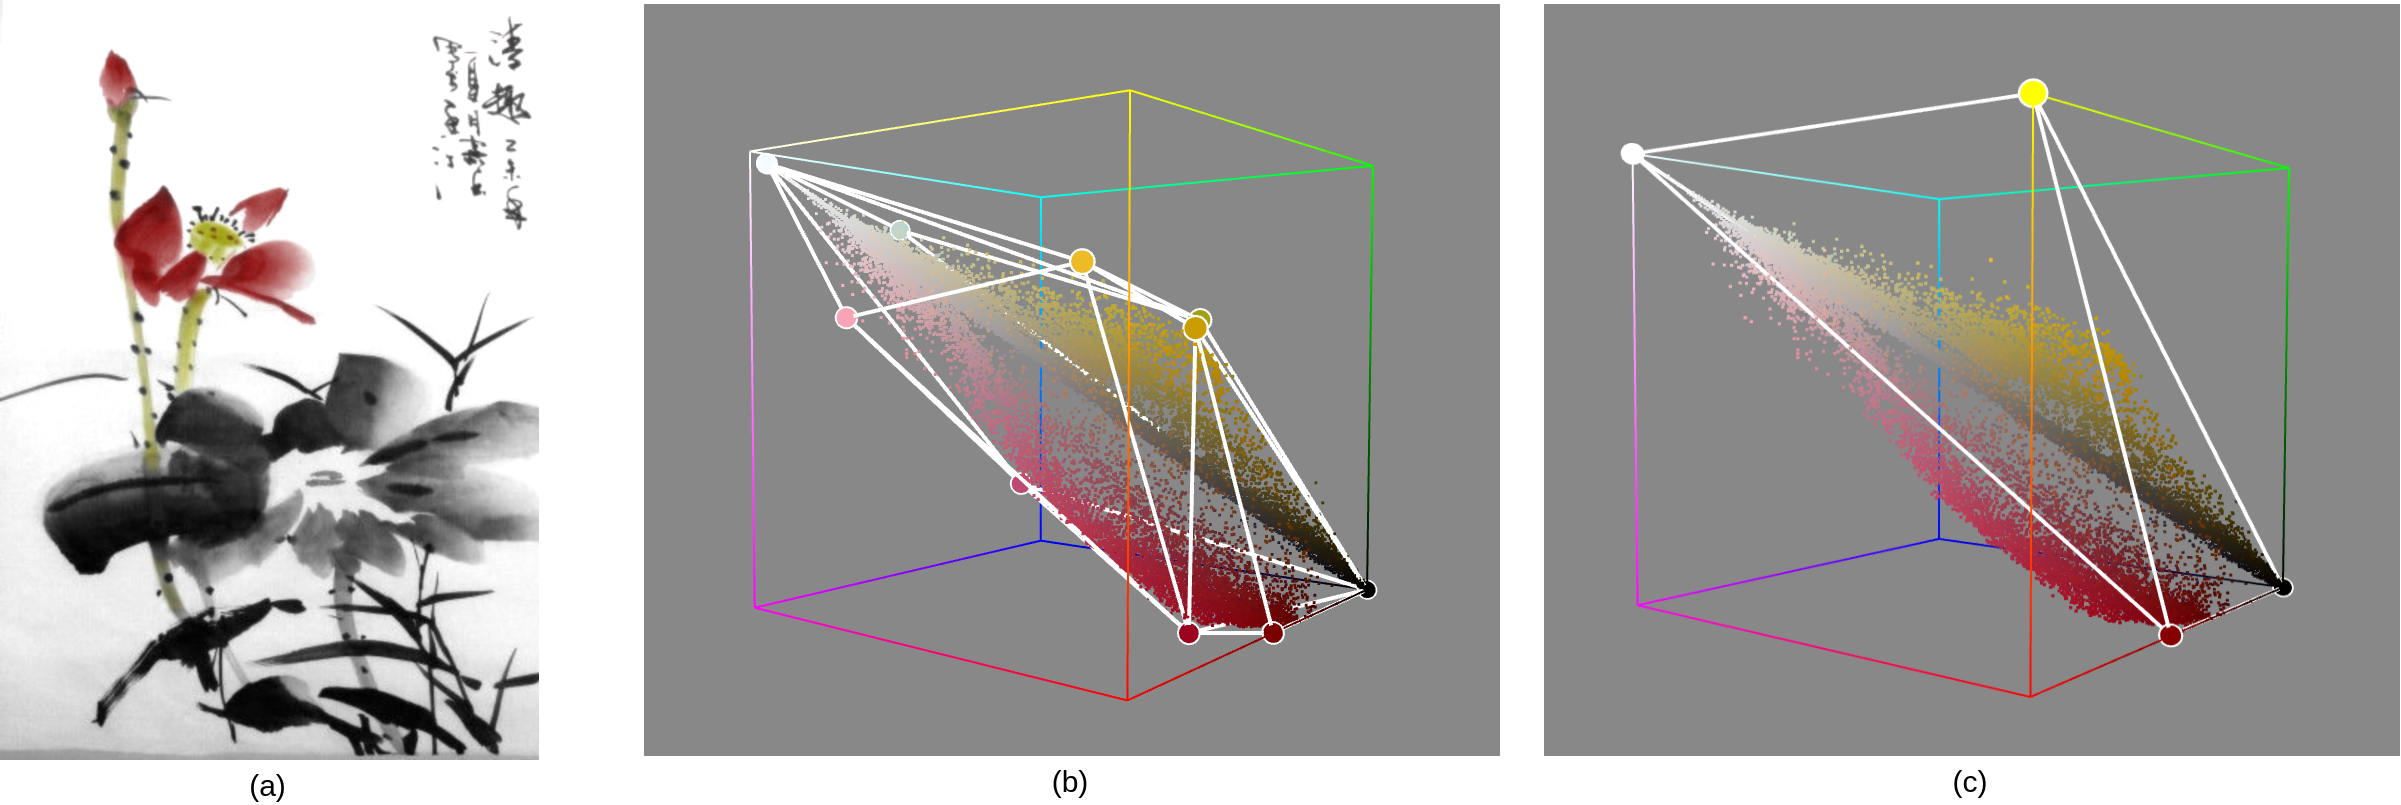
\includegraphics[height=0.18\textheight]{convex.png}
	\caption{Convex hull of input image}
	\label{convex}
	\medskip
	\small
	(a) A simple digital painting’s (b) convex hull in RGB-space is complex due to rounding. (c) The result of simplification algorithm 
\end{figure}

\section{Layer Decomposition Scheme}

\begin{figure}[H]
	\centering
	\includegraphics[height=0.2\textheight]{Layers.png}
	\caption{Decomposition layers }
	\label{decom:4layers}
\end{figure}

The standard Porter-Duff “A over B” compositing operation in \cite{porter1984compositing} is described that when the pixel $A$ with color $A_{RGB}$ and translucency $\alpha_{A}$ is placed over the pixel $B$ with color $B_{RGB}$ and translucency $\alpha_{B}$, the observed color is, 
\[  \left ( \frac{A}{B} \right )_{RGB}=\frac{\alpha_{A}A_{RGB}-(1-\alpha_{A})\alpha_{B}B_{RGB}}{\left ( \frac{A}{B} \right )_{\alpha}} \]
where 
\[\left ( \frac{A}{B} \right )_{\alpha} = \alpha_{A}+(1-\alpha_{A})\alpha_{B} \] 
Each pixel’s color is viewed as the convex combination of all layers’ colors. For each pixel, the observed color p can be approximated by the recursive application of the compositing. We take as input ordered RGB layer colors through computing per-pixel opacity values for each layer. The following ‘polynomial’ regularization term penalizes the difference between the observed color p and the polynomial approximation based on the “A over B” compositing \cite{porter1984compositing},

\[E_{polynomial}=\frac{1}{K}\left \|    C_{n}+\sum_{i=1}^{n}  \left ( \left ( C_{i-1}-C_{i} \right ) \prod_{j=i}^{n}(1-\alpha_{j}) \right )-p  \right \|^{2}\]

where $C_{i}$ denotes the i-th layer’s color, is the opacity of $\alpha_{i}$ , the background color $C_{i}$ is opaque, $K=3$ and or 4 depending on the number of channels $(RGB$ or $RGB-\alpha)$. The opacity penalty is expressed as,
\[E_{opaque}=\frac{1}{n}\sum_{i=1}^n-(1-\alpha_{i})^2\]
The default smoothness penalty is expressed as,

\[E_{spatial}=\frac{1}{n}\sum_{i=1}^n( \bigtriangledown  \alpha_{i})^2\]

where $ \bigtriangledown  \alpha_{i}$is the spatial gradient of opacity in the i-th layer. This term penalizes solutions which are not spatially smooth. However, the gradient of opacity is not always aligned with that of intensity, which may result in edges discontinuous.
The users may specify the layer order in advance, as well as the number of layers, n, is given. The opacity for every layer may be solved by minimizing the following combined cost function,
\begin{equation}
E=\omega_{polynomial}E_{polynomial}+\omega_{opaque}E_{opaque}+\omega_{spatial}E_{spatial}
\label{eq:layer1}
\end{equation} 
where $\omega_{polynomial} = 375 ,\omega_{opaque}=1 , \omega_{spatial}=10$. 

\subsection{Our Modified Layer Decomposition}
\begin{figure}[H]
	\centering
	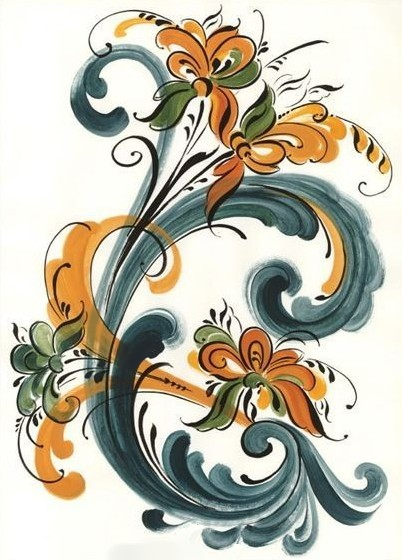
\includegraphics[width=4cm]{5.png}
	~~~~
	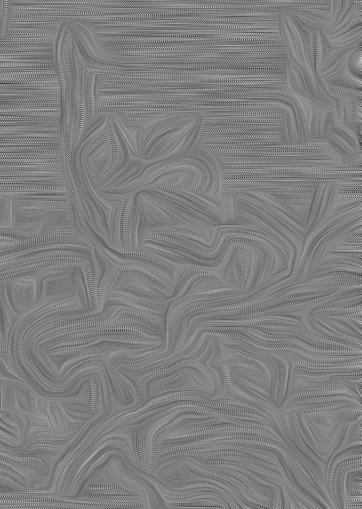
\includegraphics[width=4cm]{5etf.png}
	\caption{Edge Tangent Flow}
	\label{ETF}
\end{figure}

As we can see in Figure \ref{decom:4layers},the extracted layers failed to maintain the completeness of the brush strokes, especially in the first layer. To enhance the smoothness and completeness of extracted strokes, the coherent line drawing technique in \cite{kang2007coherent} is introduced to Eq \ref{eq:layer1} ,which is a flow-guided anisotropic filtering framework.In the coherent line drawing technique, the edge tangent flow(ETF) of a image is calculated, represented by a vector $t^{new(x)} $. Here, we use vector $t^{new(x)} $ to mimic the brush stroke direction.  Figure \ref{ETF} shows the edge tangent flow $($ETF$)$ field of a Chinese painting.\newline
The ETF field is defined as,
\begin{equation}
 t^{new(x)}=\frac{1}{k}\sum_{y\in\Omega(x)} \varphi(x,y)t^{current}(y)\omega_{s}(x,y)\omega_{m}(x,y)\omega_{d}(x,y)
 \label{eq:layer_etf} 
\end{equation}

$t(x)$ denotes the normalized tangent vector at pixel $x$, $\Omega(x)$ denotes the neighborhood of the pixel $x$, and $k$ is the term of vector normalization. The spatial weight function $\omega_{s}$ employs the radially-symmetric box filter with some radius. The magnitude weight function $\omega_{m}$ is monotonically increasing, indicating that the bigger weights are given to the neighboring pixels y whose gradient magnitudes are higher than that of the central pixel x. This ensures the preservation of the dominant edge directions. The direction weight function, $\omega_{d}$, may enhance alignment of vectors, e.g. $t(x)\cdot t(y)>0$ , while suppressing swirling flows. In addition, the sign function $\varphi(x,y)$  is employed to prevent the swirling artifact as well.

\begin{figure}[H]
	\centering
	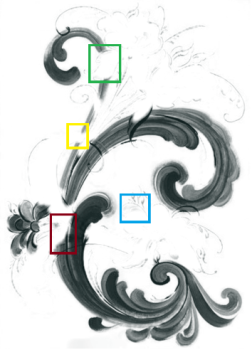
\includegraphics[width=5cm]{com_layer1.png}
	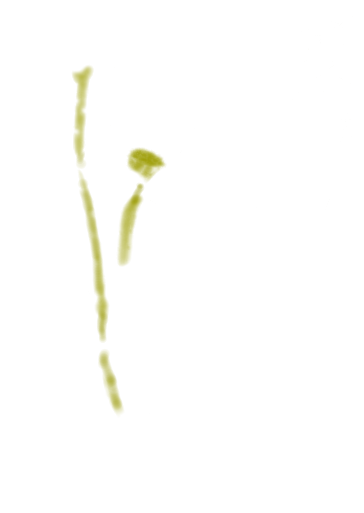
\includegraphics[width=5cm]{com_layer2.png}
	\caption{Comparison of layer decomposition  }
	\label{com eflow}
	\medskip
	\small
	Comparison of decomposed first layer before and after modification. Left shows the original result of Eq \ref{eq:layer1} , right shows the result by using $E_{flow}$ instead of $E_{spatial}$ in Eq \ref{eq:layer1}.
\end{figure}

Involving ETF filed of Eq \ref{eq:layer_etf} in $E_{spatial}$, the smoothness penalty is rewritten as,

\begin{equation} 
E_{flow}=\frac{1}{n} \sum_{i=1}^{n} \left \| t^{new} \right \| \left ( \bigtriangledown_{\theta}\alpha_{i} \right )^2 
\end{equation} 

where $\theta$ denotes the direction of $t^{new}$, and $ \bigtriangledown_{\theta}\alpha_{i} $ is the gradient of opacity in the direction of $t^{new}$. Moreover, we weight this penalty by the norm of $t^{new}$. Applying the updated $E_{flow}$ to the layer decomposition of Eq \ref{eq:layer1} instead of $E_{spatial}$, the strokes become complete and smooth, which can be noted in Figure \ref{com eflow}.

\begin{figure}[H]
	\centering
	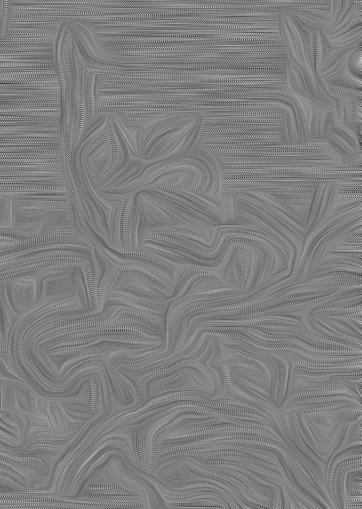
\includegraphics[width=5cm]{5etf.png}
	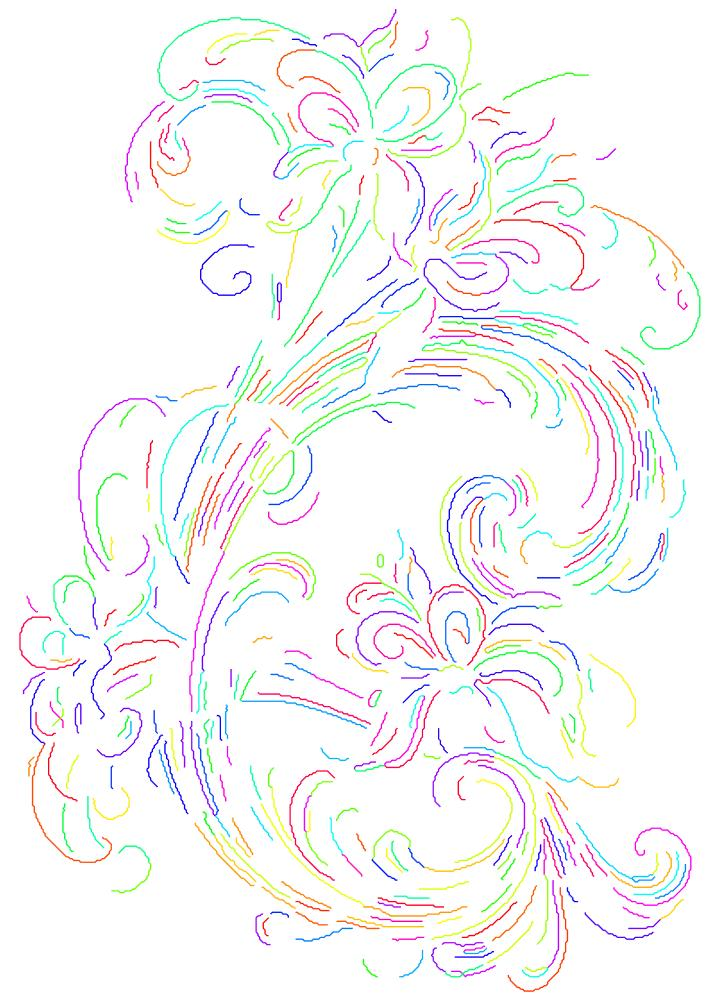
\includegraphics[width=5cm]{edge.png}
	\caption{Edge Tangent Flow field and coherent lines of the painting.}
\end{figure}


Second, the coherent lines as the constraint of brush stroke edges are involved in layer decomposition of Eq \ref{eq:layer1}. Herein, the coherent lines can be computed as follows.
\begin{figure}[H]
	\centering
	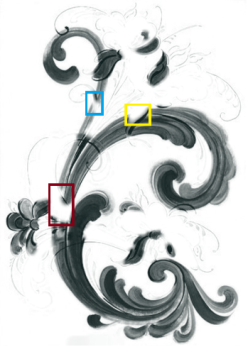
\includegraphics[width=5cm]{com_layer3.png}
	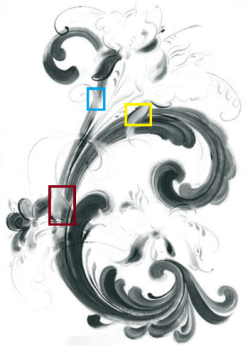
\includegraphics[width=5cm]{com_layer4.png}
	\caption{Comparison of layer decomposition before and after using $E_{egde}$  in Eq \ref{eq:layer1}; }
	\label{com:edge}
\end{figure}
Given a ETF field $t(x)$, the flow-guided anisotropic Difference of Gaussian (DoG) filter is employed, in which the kernel shape is defined by the local flow encoded in ETF field. Note that $t(x)$ represents the local edge direction. It is most likely to make the highest contrast in the perpendicular direction, that is, the gradient direction. When moving along the edge flow, the DoG filter is applied in the gradient direction. As a result, we can ‘exaggerate’ the filter output along genuine edges, while ‘attenuating’ the output from spurious edges. This not only enhances the coherence of the edges, but also suppresses noises. Iteratively applying this flow-based DoG filter results in a binary output which reaches a satisfactory level of line connectivity and illustration quality. The coherent lines can be regarded as the edges of brush strokes.

\begin{figure}[H]
 		\centering
	\begin{subfigure}[b]{0.4\textwidth}
		\centering
		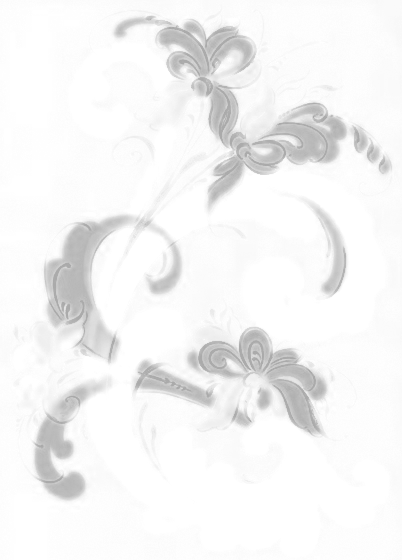
\includegraphics[width=\textwidth]{intensity.png}
		\caption{intensity map of layer2}
	\end{subfigure}
	~
	\begin{subfigure}[b]{0.4\textwidth}
		\centering
		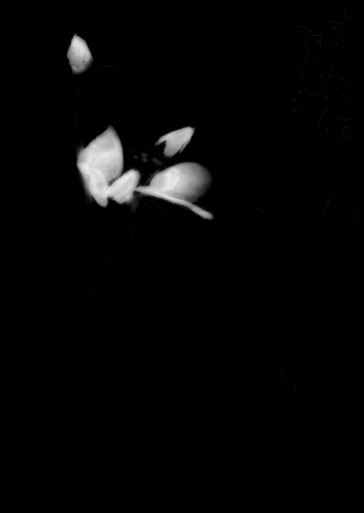
\includegraphics[width=\textwidth]{alpha.png}
		\caption{alpha map of layer2}
	\end{subfigure}
 

 
	\centering
	\begin{subfigure}[b]{0.4\textwidth}
		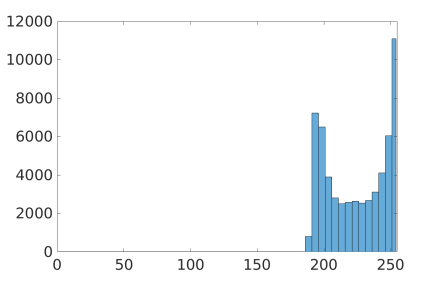
\includegraphics[clip,width=\textwidth]{h1.png}
		\caption{histogram of intensity map of layer2}
	\end{subfigure}
	~  	
	\begin{subfigure}[b]{0.4\textwidth}
		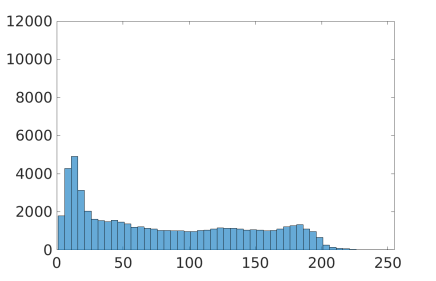
\includegraphics[clip,width=\textwidth]{h2.png}
		\caption{histogram of alpha map of layer2}
	\end{subfigure}
	\caption{Comparison between transparency and intensity of layer2}
	\label{histo}
\end{figure}
 
To preserve the stroke edges, we assume that the opacity along the coherent lines is consistent, i.e. $min \int_{l}\Arrowvert \bigtriangledown\alpha \Arrowvert^2 dx $, where l denotes the collection of coherent lines. Hence, the constraint term is defined by applying Laplacian operator to the opacity along the coherent lines,

\begin{equation} 
E_{edge}=\Arrowvert LY \Arrowvert^2 
\end{equation} 

where all the opacity $\alpha_i$ are stacked in the vector $Y$, and $L$ denotes the connection matrix. The eight-connected neighboring rule is utilized to construct the connection matrix $L$, that is, if two adjacent pixels, i and j, stay on the same coherent line, the item of $L(i,j)$ is set to -1 ; otherwise 0. Figure \ref{com:edge}a and \ref{com:edge}b shows that the edges of strokes become visible and complete after involving $E_{edge}$ into Eq \ref{eq:layer1}.
Accordingly, the layer decomposition of Eq \ref{eq:layer1} is rewritten as,

\begin{equation}
E=\omega_{polynomial}E_{polynomial}+\omega_{opaque}E_{opaque}+\omega_{flow}E_{flow}+\omega_{edge}E_{edge}
\label{eq:layer_sum}
\end{equation} 

We select the value of weights based on calculate the root-mean-square-error (RMSE) of the opacity of the coherent lines on each layer.By minimizing the RMSE, we set $\omega_{polynomial}=365, \omega_{opaque}=0.1,\omega_{flow}=100, \omega_{edge}=20 $ . 
\section{Comparison of layer decompostion} \label{comparelayer}
To demonstrate our results can better preserve the smoothness and completeness of brush strokes, we perform the schemes of Eq \ref{eq:layer1} and Eq \ref{eq:layer_sum} separately on the same set of  paintings and compare the root-mean-square-error (RMSE) of the opacity of the coherent lines on each layer shown in Table 1. The RMSE by Eq \ref{eq:layer_sum} is noticeably less than that by Eq \ref{eq:layer1}. This means that the coherent lines have been embedded into the opacity of each layer. As we mentioned, the weights in equation \ref{eq:layer_sum} are empirically determined in terms of the opacity RMSE of coherent lines. \\
To demonstrate the robustness of our approach, including Chinese paintings, we also perform the comparison on some other paintings with highly characteristic brush strokes, such as rosemailing paintings\cite{ellingsgard1978rosemaling} and Vincent van Gogh's paintings\cite{li2012rhythmic} . 

\begin{figure}
	\centering
	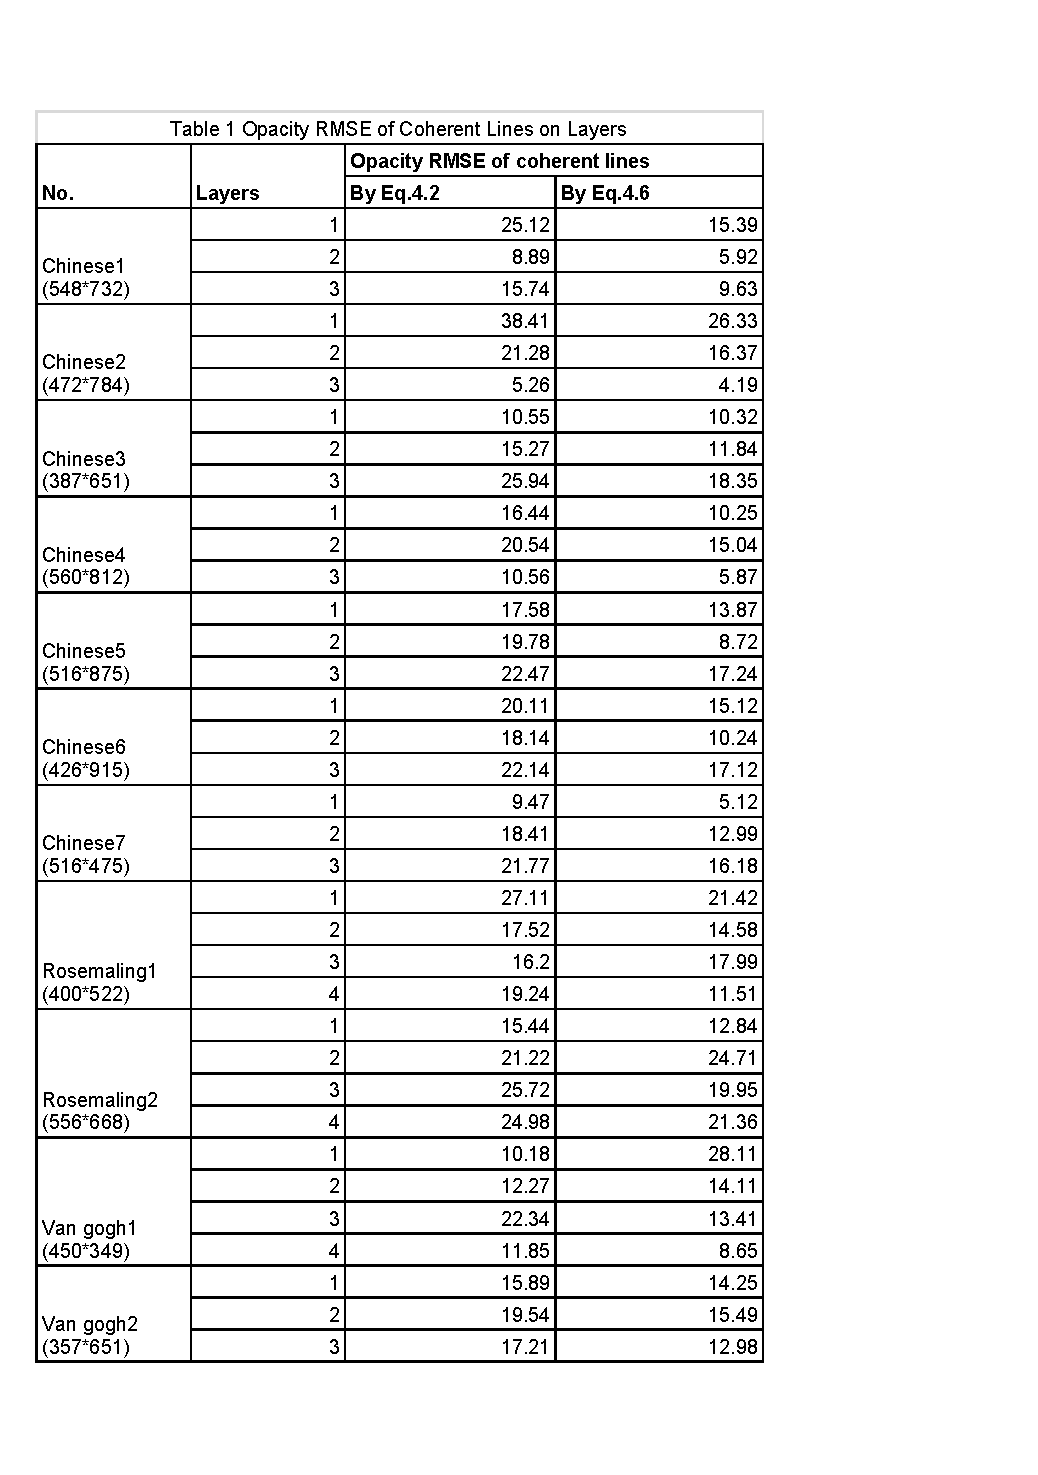
\includegraphics[width=17cm]{rmse.pdf}
	\label{table1}

\end{figure}

















